% Provenance (never printed): see sources/outline_sources.md (Year 1: the wind-driven
% circulation, gyres, Ekman transport and upwelling, western boundary currents, the
% meridional overturning circulation and the water masses). Exercise and problem values in
% the Book 3 scratch calculator calc/ch29.py; figures from figdata/bachelor-1/
% ekman_hodograph.py (Ekman's solution with Ekman's constants) and stommel_gyre.py
% (Stommel's 1948 model, exercise parameters), the world map from figdata/shared/geo.py.
% Physics owns the Coriolis force (recalled). Book 1 (g8) gave the surface currents and
% the gyres in words, Book 2 (g10) upwelling: re-founded here with the Ekman balance.
% Ch. 26 owns the T-S diagram and the water masses, ch. 28 the Coriolis parameter, the
% geostrophic wind and the mean meridional streamfunction. The Sverdrup balance, the
% vorticity argument and the derivation of the Ekman spiral are the Year 3 volume's; ENSO
% the Year 2 volume's.
\chapter{A circulação do oceano}\label{ch:b1:ocean-circulation}

Em 1992, durante uma tempestade no Pacífico Norte, um contêiner caiu ao mar de um navio que seguia de
Hong Kong para os Estados Unidos. Ele se abriu e liberou cerca de \num{29000} patos de borracha e outros
brinquedos de banho, que flutuaram para longe e viajaram por grandes distâncias; os lugares onde alguns
deles foram encontrados depois ajudaram os cientistas a entender as correntes que os tinham levado.
Brinquedos flutuantes seguem a água da superfície, e a água superficial dos oceanos não vagueia ao
acaso: ela gira em \omterm{def:b1:ocean-circulation:gyre}{giros} de escala de bacia, corre para o norte em correntes estreitas ao longo das
costas ocidentais dos oceanos, e sobe ou desce em alguns poucos lugares escolhidos. Este capítulo
explica como o vento põe a parte superior do oceano em movimento, por que a água se move em ângulo
reto com o vento que a empurra, por que as correntes mais fortes se encostam nos lados ocidentais dos
oceanos, e como uma lenta circulação de inversão leva água para o abismo e de volta.
% ledger: noaa:floatees

\begin{omfigure}
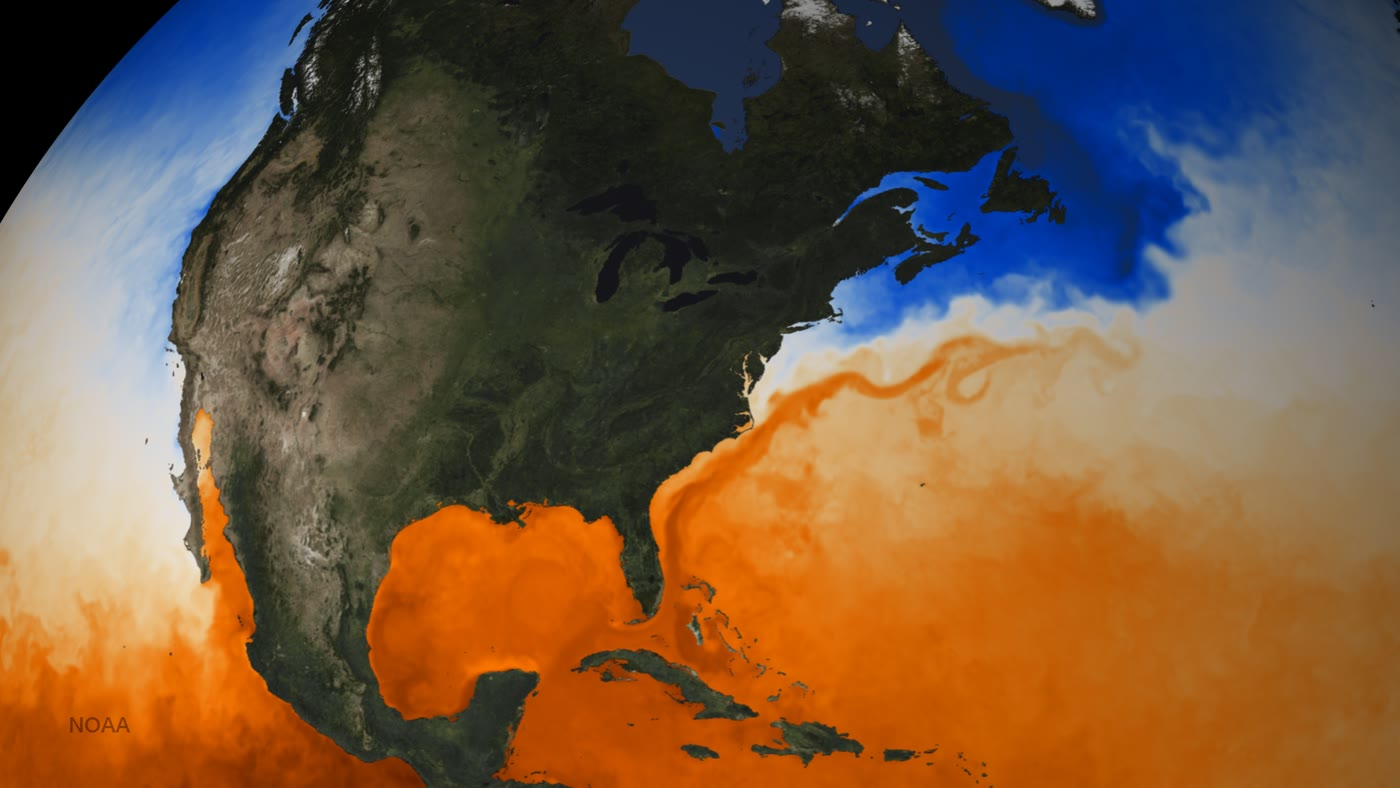
\includegraphics[width=0.85\linewidth]{images/book3/b1-gulf-stream-sst.jpg}

{\small A temperatura da superfície do mar em torno da América do Norte no início de junho de 2016, a
partir de dados de satélite (água quente em laranja, água fria em azul). A Corrente do Golfo sai da
costa dos Estados Unidos como uma fita quente e sinuosa e atravessa o Atlântico rumo à Europa; nas
mesmas \omterm{def:b1:spherical-astronomy:geographic}{latitudes}, a água ao largo da costa do Pacífico é bem mais fria que ao largo da costa do
Atlântico. (NOAA, NESDIS, domínio público, via Wikimedia Commons.)}
\label{fig:b1:ocean-circulation:sst}
\end{omfigure}
% ledger: commons:gulf-stream-sst, noaa:gulf-stream-heat

\begin{recall}
Os livros de física dão a força de Coriolis. \Cref{ch:b1:atmospheric-circulation} escreveu sua parte
horizontal como $-f\,\vec k\times\vec v$, com o \omterm{def:b1:atmospheric-circulation:coriolis-parameter}{parâmetro de Coriolis} $f = 2\Omega\sin\varphi$
($\Omega = \qty{7.292e-5}{rad.s^{-1}}$), e encontrou os \omterm{def:b1:atmospheric-circulation:winds}{alísios}, leste entre o equador e cerca de
\ang{30}, e os \omterm{def:b1:atmospheric-circulation:winds}{ventos de oeste} além; também definiu a \omterm{def:b1:atmospheric-circulation:streamfunction}{função de corrente meridional média} de uma
inversão. \Cref{ch:b1:fluid-envelopes-structure} deu a \omterm{def:b1:fluid-envelopes-structure:ocean-layers}{camada de mistura} e a \omterm{def:b1:fluid-envelopes-structure:ocean-layers}{termoclina}, a densidade da
água do mar, o \omterm{def:b1:fluid-envelopes-structure:ts-diagram}{diagrama T--S} e as \omterm{def:b1:fluid-envelopes-structure:ts-diagram}{massas de água} do Atlântico Sul, e \cref{ch:b1:radiation-heat-transport}
o transporte de calor para os polos partilhado pela atmosfera e pelo oceano. O Livro~1 descreveu as
correntes superficiais e os grandes \omterm{def:b1:ocean-circulation:gyre}{giros}; o Livro~2, a \omterm{def:b1:ocean-circulation:upwelling}{ressurgência} de água fria ao longo de algumas costas.
% ledger: earth:Trot, nos:gyres
\end{recall}

\section{O vento e as correntes superficiais}\label{sec:b1:ocean-circulation:wind}

O vento move o mar roçando nele. Sua força se espalha pela superfície, e é medida, como uma pressão,
por unidade de área.

\begin{definition}[Tensão do vento]\label{def:b1:ocean-circulation:wind-stress}
A \emph{tensão do vento}\index{tensão do vento} $\vec T$ é a força horizontal por unidade de área
exercida pelo vento sobre a superfície do mar, em pascals. É a transferência para baixo do momento
horizontal do ar para o oceano, e aponta quase na direção do vento. Seu tamanho é dado pela fórmula aerodinâmica
\[
  T = \rho_a C_D U_{10}^2,
\]
onde $\rho_a = \qty{1.3}{kg.m^{-3}}$ é a densidade do ar, $U_{10}$ a velocidade do vento a
\qty{10}{m} acima do mar e $C_D$ um coeficiente de arrasto adimensional.
\end{definition}
% ledger: stewart:wind-stress

O coeficiente de arrasto é medido com instrumentos rápidos que registram as flutuações turbulentas do
vento a alguns metros acima das ondas. Para um ar de estabilidade neutra, as medidas de Yelland e Taylor dão
\[
  1000\,C_D = 0.29 + \frac{3.1}{U_{10}} + \frac{7.7}{U_{10}^2}
  \quad (\qtyrange{3}{6}{m/s}),
  \qquad
  1000\,C_D = 0.60 + 0.071\,U_{10}
  \quad (\qtyrange{6}{26}{m/s}),
\]
com $U_{10}$ em metros por segundo. Um vento de \qty{10}{m/s} tem $C_D =
\num{1.31e-3}$ e exerce $T = 1.3 \times \num{1.31e-3} \times 100 =
\qty{0.170}{Pa}$; um vento de \qty{5}{m/s}, \qty{0.040}{Pa}; um vendaval de
\qty{20}{m/s}, \qty{1.05}{Pa}. Dobrar o vento de 10 para \qty{20}{m/s} multiplica a tensão por $6.2$,
não por $4$: mares mais ásperos agarram o vento com mais força. Essas tensões são minúsculas, uma
milionésima parte da pressão atmosférica, mas agem sem pausa sobre todo o oceano.
% ledger: stewart:drag-coefficient (computed in figdata/bachelor-1/ekman_hodograph.py and calc/ch29.py)

A forma da tensão segue a dos ventos. Entre os \omterm{def:b1:atmospheric-circulation:winds}{alísios} dos trópicos, que sopram para oeste, e os \omterm{def:b1:atmospheric-circulation:winds}{ventos
de oeste} das \omterm{def:b1:spherical-astronomy:geographic}{latitudes} médias, que sopram para leste, a água superficial de cada bacia oceânica é posta
a girar.

\begin{definition}[Giro; giros subtropical e subpolar]\label{def:b1:ocean-circulation:gyre}
Um \emph{giro}\index{giro} é um grande sistema de correntes oceânicas em rotação que preenche uma bacia
oceânica. Um \emph{giro subtropical}\index{giro subtropical} fica entre os \omterm{def:b1:atmospheric-circulation:winds}{alísios} e os \omterm{def:b1:atmospheric-circulation:winds}{ventos de oeste} e
gira no sentido horário no Hemisfério Norte e no sentido anti-horário no Sul. Um \emph{giro subpolar}\index{giro subpolar}
fica no lado polar dos \omterm{def:b1:atmospheric-circulation:winds}{ventos de oeste} e gira no sentido contrário.
\end{definition}
% ledger: nos:gyre-def, nos:boundary-currents, stewart:north-atlantic

Há cinco \omterm{def:b1:ocean-circulation:gyre}{giros} subtropicais, no Atlântico Norte e Sul, no Pacífico Norte e Sul e no Índico; nenhum
atravessa o equador. No Atlântico Norte, o \omterm{def:b1:ocean-circulation:gyre}{giro subtropical} é fechado pela Corrente do Golfo ao longo da
costa dos Estados Unidos, a oeste, e pela Corrente das Canárias ao largo da África, a leste; ao norte
dele, o \omterm{def:b1:ocean-circulation:gyre}{giro subpolar} gira no sentido anti-horário, com a Corrente do Atlântico Norte em seu lado sul e a
Corrente do Labrador fluindo para o sul ao longo de seu lado ocidental. Em baixas \omterm{def:b1:spherical-astronomy:geographic}{latitudes}, as correntes
equatoriais de oeste do Atlântico e do Pacífico são separadas por uma contracorrente de leste. Os \omterm{def:b1:ocean-circulation:gyre}{giros} não
são simétricos: cada \omterm{def:b1:ocean-circulation:gyre}{giro subtropical} é fechado por uma corrente forte e estreita do lado ocidental de sua
bacia e por uma corrente fraca e larga do lado oriental. Em torno da Antártida, onde nenhum continente a
detém, a Corrente Circumpolar Antártica flui para leste ao redor do globo, impelida pelos \omterm{def:b1:atmospheric-circulation:winds}{ventos de oeste}
do Oceano Austral.
% ledger: nos:boundary-currents, stewart:north-atlantic, stewart:heat-conveyor, lien:kuroshio, donohue:acc, stewart:acc

\begin{omfigure}
\begin{tikzpicture}
\begin{axis}[ommap, width=0.98\linewidth, xtick={-180,-120,...,180}, ytick={-60,-30,0,30,60}]
% land: figdata/shared/geo.py; ledger: data:ne-land. Arrows placed by hand from the
% ledgered pattern: nos:boundary-currents, stewart:north-atlantic, lien:kuroshio,
% donohue:acc, stewart:acc
\addplot[fill=omLithAlluv, draw=black!45, line width=0.2pt, forget plot] table {figdata/out/shared-geo-land.dat};
% North Atlantic subtropical gyre (clockwise)
\addplot[omThm, line width=1.1pt, -{Stealth[length=4pt]}, smooth] coordinates {(-80,26) (-77,32) (-70,37) (-58,40) (-44,41)};
\addplot[omThm, line width=1.1pt, -{Stealth[length=4pt]}, smooth] coordinates {(-38,40) (-28,39) (-20,36)};
\addplot[omThm, line width=1.1pt, -{Stealth[length=4pt]}, smooth] coordinates {(-19,32) (-21,24) (-26,17)};
\addplot[omThm, line width=1.1pt, -{Stealth[length=4pt]}, smooth] coordinates {(-32,14) (-45,13) (-60,15)};
% North Atlantic subpolar gyre (anticlockwise)
\addplot[omDef, line width=1.1pt, -{Stealth[length=4pt]}, smooth] coordinates {(-40,47) (-28,52) (-18,57)};
\addplot[omDef, line width=1.1pt, -{Stealth[length=4pt]}, smooth] coordinates {(-24,61) (-35,62) (-44,59)};
\addplot[omDef, line width=1.1pt, -{Stealth[length=4pt]}, smooth] coordinates {(-55,59) (-56,53) (-51,47)};
% North Pacific subtropical gyre (clockwise)
\addplot[omThm, line width=1.1pt, -{Stealth[length=4pt]}, smooth] coordinates {(123,19) (125,26) (133,32) (143,36) (156,38)};
\addplot[omThm, line width=1.1pt, smooth] coordinates {(162,39) (172,40) (180,40.5)};
\addplot[omThm, line width=1.1pt, -{Stealth[length=4pt]}, smooth] coordinates {(-180,40.5) (-165,41) (-148,40)};
\addplot[omThm, line width=1.1pt, -{Stealth[length=4pt]}, smooth] coordinates {(-133,37) (-128,29) (-122,20)};
\addplot[omThm, line width=1.1pt, -{Stealth[length=4pt]}, smooth] coordinates {(-125,13) (-150,12) (-175,13)};
\addplot[omThm, line width=1.1pt, -{Stealth[length=4pt]}, smooth] coordinates {(170,13) (152,14) (135,15)};
% South Atlantic subtropical gyre (anticlockwise)
\addplot[omThm, line width=1.1pt, -{Stealth[length=4pt]}, smooth] coordinates {(2,-8) (-15,-9) (-30,-9)};
\addplot[omThm, line width=1.1pt, -{Stealth[length=4pt]}, smooth] coordinates {(-34,-14) (-39,-24) (-47,-34)};
\addplot[omThm, line width=1.1pt, -{Stealth[length=4pt]}, smooth] coordinates {(-42,-40) (-20,-40) (2,-38)};
\addplot[omThm, line width=1.1pt, -{Stealth[length=4pt]}, smooth] coordinates {(10,-31) (9,-23) (6,-15)};
% South Pacific subtropical gyre (anticlockwise)
\addplot[omThm, line width=1.1pt, -{Stealth[length=4pt]}, smooth] coordinates {(-88,-10) (-120,-11) (-160,-12)};
\addplot[omThm, line width=1.1pt, -{Stealth[length=4pt]}, smooth] coordinates {(160,-16) (157,-26) (162,-35)};
\addplot[omThm, line width=1.1pt, -{Stealth[length=4pt]}, smooth] coordinates {(-170,-40) (-140,-41) (-105,-39)};
\addplot[omThm, line width=1.1pt, -{Stealth[length=4pt]}, smooth] coordinates {(-82,-36) (-82,-27) (-85,-17)};
% Indian Ocean subtropical gyre (anticlockwise)
\addplot[omThm, line width=1.1pt, -{Stealth[length=4pt]}, smooth] coordinates {(98,-13) (80,-14) (60,-15)};
\addplot[omThm, line width=1.1pt, -{Stealth[length=4pt]}, smooth] coordinates {(47,-22) (40,-29) (33,-34)};
\addplot[omThm, line width=1.1pt, -{Stealth[length=4pt]}, smooth] coordinates {(50,-38) (75,-37) (100,-35)};
\addplot[omThm, line width=1.1pt, -{Stealth[length=4pt]}, smooth] coordinates {(108,-31) (106,-24) (102,-18)};
% Antarctic Circumpolar Current (eastward)
\addplot[omMeth, line width=1.4pt, -{Stealth[length=5pt]}, smooth] coordinates {(-62,-58) (-40,-55) (-15,-52)};
\addplot[omMeth, line width=1.4pt, -{Stealth[length=5pt]}, smooth] coordinates {(5,-52) (40,-50) (75,-50)};
\addplot[omMeth, line width=1.4pt, -{Stealth[length=5pt]}, smooth] coordinates {(95,-51) (130,-53) (165,-56)};
\addplot[omMeth, line width=1.4pt, -{Stealth[length=5pt]}, smooth] coordinates {(-170,-58) (-130,-59) (-85,-59)};
\node[font=\scriptsize, anchor=west, fill=white, fill opacity=0.8, text opacity=1, inner sep=1pt] at (axis cs:-66,31) {Corrente do Golfo};
\node[font=\scriptsize, anchor=west, fill=white, fill opacity=0.8, text opacity=1, inner sep=1pt] at (axis cs:-11,25) {Canárias};
\node[font=\scriptsize, anchor=east, fill=white, fill opacity=0.8, text opacity=1, inner sep=1pt] at (axis cs:-58,52) {Labrador};
\node[font=\scriptsize, anchor=west, fill=white, fill opacity=0.8, text opacity=1, inner sep=1pt] at (axis cs:142,28) {Kuroshio};
\node[font=\scriptsize, anchor=north, fill=white, fill opacity=0.8, text opacity=1, inner sep=1pt] at (axis cs:-150,9) {Equatorial Norte};
\node[font=\scriptsize, anchor=north, fill=white, fill opacity=0.8, text opacity=1, inner sep=1pt] at (axis cs:0,-62) {Corrente Circumpolar Antártica};
\end{axis}
\end{tikzpicture}

{\small Os \omterm{def:b1:ocean-circulation:gyre}{giros} da superfície do oceano (setas esquemáticas sobre um mapa das terras). Vermelho escuro:
os cinco \omterm{def:b1:ocean-circulation:gyre}{giros} subtropicais, no sentido horário no Hemisfério Norte e anti-horário no Sul, cada um com
uma corrente de contorno ocidental estreita; azul: o \omterm{def:b1:ocean-circulation:gyre}{giro subpolar} do Atlântico Norte; verde: a Corrente
Circumpolar Antártica. Nomeadas estão apenas as correntes discutidas no texto. As setas mostram o sentido
do escoamento, não sua velocidade.}
\label{fig:b1:ocean-circulation:gyres}
\end{omfigure}
% ledger: data:ne-land, nos:boundary-currents, stewart:north-atlantic, lien:kuroshio, donohue:acc

Dois aspectos desse padrão precisam de explicação. O primeiro é o sentido da rotação: os \omterm{def:b1:atmospheric-circulation:winds}{alísios} sopram
para oeste no lado equatorial de um \omterm{def:b1:ocean-circulation:gyre}{giro subtropical}, mas as correntes do \omterm{def:b1:ocean-circulation:gyre}{giro} não seguem simplesmente os
ventos, e a água superficial deriva em um ângulo com eles. O segundo é a assimetria: o escoamento de
retorno de um \omterm{def:b1:ocean-circulation:gyre}{giro} é comprimido contra o lado ocidental de sua bacia. Ambos vêm da rotação da Terra.

\section{Transporte de Ekman}\label{sec:b1:ocean-circulation:ekman}

\begin{history}[Nansen e Ekman, 1898--1905]
Durante sua expedição no Ártico, Fridtjof Nansen notou que o vento empurrava o gelo marinho não na
direção do vento, mas em um ângulo de \ang{20} a \ang{40} à sua direita, olhando a favor do vento. Ele
raciocinou que três forças tinham de se equilibrar sobre o gelo em movimento: o empurrão do vento, o
atrito da água e a força de Coriolis. Pediu ao meteorologista Vilhelm Bjerknes que deixasse um de seus
alunos estudar a influência da rotação da Terra sobre as correntes induzidas pelo vento. O aluno, Walfrid
Ekman, desenvolveu a teoria para sua tese de doutorado em Uppsala, e a estendeu em 1905. Sua solução
ainda é o ponto de partida da teoria do oceano movido pelo vento.
\end{history}
% ledger: stewart:ekman-layer, nos:ekman-spiral

\begin{definition}[Camada de Ekman, transporte de Ekman, espiral de Ekman]\label{def:b1:ocean-circulation:ekman}
A \emph{camada de Ekman}\index{camada de Ekman} é a fina camada superficial do oceano, de no máximo
algumas centenas de metros de espessura, na qual a \omterm{def:b1:ocean-circulation:wind-stress}{tensão do vento} é levada para baixo pelo atrito
turbulento e equilibrada pela força de Coriolis. O \emph{transporte de Ekman}\index{transporte de Ekman}
é a \omterm{def:b1:fluid-envelopes-structure:ts-diagram}{massa de água} que a camada leva por segundo através de uma faixa vertical de \qty{1}{m} de largura,
da superfície até abaixo da camada:
\[
  \vec M = \int_{-d}^{0} \rho\,\vec v\,\mathrm dz \quad (\unit{kg.m^{-1}.s^{-1}});
\]
dividida pela densidade, é um transporte volumétrico por metro, em \unit{m^2.s^{-1}}. A \emph{espiral de
Ekman}\index{espiral de Ekman} é o \omterm{def:b1:ocean-circulation:gyre}{giro} e o enfraquecimento da corrente com a profundidade na camada.
Os transportes oceânicos são contados em \emph{sverdrups}\index{sverdrup (unidade)}: \qty{1}{\sverdrup} $=
\qty{e6}{m^3.s^{-1}}$.
\end{definition}
% ledger: stewart:ekman-layer, stewart:ekman-transport

\begin{theorem}[Transporte de Ekman]\label{thm:b1:ocean-circulation:ekman}
Em regime permanente, longe das costas, sobre água muito mais profunda que a \omterm{def:b1:ocean-circulation:ekman}{camada de Ekman}, o
\omterm{def:b1:ocean-circulation:ekman}{transporte de Ekman} depende apenas da \omterm{def:b1:ocean-circulation:wind-stress}{tensão do vento} $\vec T$ e do \omterm{def:b1:atmospheric-circulation:coriolis-parameter}{parâmetro de Coriolis} $f$:
\[
  \vec M = \frac{1}{f}\,\vec T\times\vec k,
  \qquad |\vec M| = \frac{|\vec T|}{|f|}.
\]
Ele é perpendicular à \omterm{def:b1:ocean-circulation:wind-stress}{tensão do vento}, à sua direita no Hemisfério Norte e à sua esquerda no Sul.
\end{theorem}
% ledger: stewart:ekman-transport

\begin{proof}
Seja $\vec\tau(z)$ a tensão de cisalhamento horizontal que a água acima do nível $z$
exerce sobre a água abaixo dele. Na superfície, ela é a \omterm{def:b1:ocean-circulation:wind-stress}{tensão do vento}, $\vec\tau(0) =
\vec T$; abaixo da camada, onde as correntes geradas pelo vento já se extinguiram, ela
se anula, $\vec\tau(-d) = \vec 0$. Uma fina lâmina entre $z$ e $z + \mathrm dz$, de área
horizontal unitária, recebe $\vec\tau(z + \mathrm dz)$ em sua face superior e
$-\vec\tau(z)$ em sua face inferior: a força de atrito resultante é $(\partial\vec
\tau/\partial z)\,\mathrm dz$. Sua massa é $\rho\,\mathrm dz$, e a força de Coriolis
horizontal sobre ela é $-f\,\vec k\times\vec v\,\rho\,\mathrm dz$. Em regime
permanente, sem variação horizontal de um lugar para outro, as duas se equilibram:
\[
  -f\rho\,\vec k\times\vec v + \frac{\partial\vec\tau}{\partial z} = \vec 0 .
\]
Integrando de $-d$ a $0$,
\[
  -f\,\vec k\times\vec M + \vec\tau(0) - \vec\tau(-d) = \vec 0,
  \qquad\text{ou seja}\qquad \vec k\times\vec M = \frac{\vec T}{f}.
\]
Para um vetor horizontal, $\vec k\times(\vec k\times\vec M) = -\vec M$; tomando
$\vec k\times$ de ambos os lados dá $-\vec M = \vec k\times\vec T/f$, logo $\vec M =
\vec T\times\vec k/f$. O vetor $\vec T\times\vec k$ é $\vec T$ girado de
\ang{90} no sentido horário visto de cima: à direita do vento quando $f > 0$, à
esquerda quando $f < 0$. Seu módulo é $|\vec T|$.
\end{proof}

O resultado não depende de como o atrito funciona dentro da camada, que é
pouco conhecido: só entram a tensão no topo e seu desaparecimento na base.
Isso torna o transporte muito mais robusto do que as próprias velocidades. A água
de toda a camada, tomada em conjunto, move-se em ângulo reto com o vento, um resultado que
parece estranho até lembrar que, ao longo de um dia ou mais, a força de Coriolis tem
tempo de girar cada corrente.

\begin{example}[O transporte sob uma brisa fresca]\label{ex:b1:ocean-circulation:transport}
Um vento de \qty{10}{m/s} soprando para o norte a \ang{35} N exerce
$T = \qty{0.170}{Pa}$. Com $f = 2\Omega\sin\ang{35} = \qty{8.365e-5}{s^{-1}}$, o
\omterm{def:b1:ocean-circulation:ekman}{transporte de Ekman} é $0.170/(\num{8.365e-5}) = \qty{2036}{kg.m^{-1}.s^{-1}}$, para
leste. Com $\rho = \qty{1027}{kg.m^{-3}}$, isso dá \qty{1.98}{m^3.s^{-1}} para
cada metro medido através do transporte: através de uma linha de \qty{1000}{km} de comprimento, cerca de
\qty{2}{\sverdrup}.
\end{example}
% ledger: stewart:drag-coefficient, stewart:ekman-constants, earth:Trot (computed in calc/ch29.py)

O teorema foi testado no mar. Em \ang{11} N no Atlântico, onde os
\omterm{def:b1:atmospheric-circulation:winds}{alísios} sopram para oeste, o \omterm{def:b1:ocean-circulation:ekman}{transporte de Ekman} é para o norte; medido
diretamente com um perfilador de correntes, deu
\qty[uncertainty-mode=separate]{12.0 \pm 5.5}{\sverdrup}, contra
\qty[uncertainty-mode=separate]{8.8 \pm 1.9}{\sverdrup} calculado a partir dos ventos
medidos durante a campanha e
\qty[uncertainty-mode=separate]{13.5 \pm 0.3}{\sverdrup} a partir de ventos médios ao longo de
muitos anos.
% ledger: stewart:ekman-transport

Como a corrente se distribui em profundidade dentro da camada depende do
atrito. Ekman adotou o modelo mais simples, um atrito turbulento proporcional ao
cisalhamento vertical da corrente, $\vec\tau = \rho A_z\,\partial\vec v/\partial z$, com
uma viscosidade turbulenta constante $A_z$.

\begin{proposition}[A espiral de Ekman]\label{prop:b1:ocean-circulation:spiral}
Para uma \omterm{def:b1:ocean-circulation:wind-stress}{tensão do vento} $T$ permanente, dirigida para o norte sobre um oceano profundo e homogêneo no
Hemisfério Norte, com viscosidade turbulenta constante $A_z$, a corrente à altura $z
\leq 0$ é
\[
  u = V_0\,e^{az}\cos\Bigl(\frac\pi4 + az\Bigr),\qquad
  v = V_0\,e^{az}\sin\Bigl(\frac\pi4 + az\Bigr),\qquad
  a = \sqrt{\frac{f}{2A_z}},\quad V_0 = \frac{T}{\rho\sqrt{fA_z}},
\]
com $u$ para leste e $v$ para o norte. Na superfície, a corrente flui a \ang{45} à
direita do vento; com a profundidade ela enfraquece como $e^{az}$ e gira ainda mais para a
direita. Na profundidade $D_E = \pi/a$, a profundidade de Ekman, ela flui em sentido
oposto ao da corrente da superfície, com $e^{-\pi} = \num{0.043}$ de sua velocidade.
\end{proposition}
\admitted
% ledger: stewart:ekman-solution

A dedução resolve as duas equações $f v + A_z u'' = 0$ e $-f u + A_z v'' =
0$ do equilíbrio da demonstração acima; ela é feita no volume do terceiro ano, e
\cref{exo:b1:ocean-circulation:10} verifica que as fórmulas satisfazem as equações
e que a espiral transporta exatamente o transporte do teorema. Para usar a
espiral, é preciso $A_z$, que não é medido diretamente. Ekman reuniu as
velocidades observadas das correntes de superfície e encontrou, para $|\varphi| \geq \ang{10}$,
\[
  V_0 = \frac{0.0127\,U_{10}}{\sqrt{\sin|\varphi|}},
  \qquad\text{donde}\qquad
  D_E = \frac{7.6\,U_{10}}{\sqrt{\sin|\varphi|}},
\]
em unidades SI, com seu coeficiente de arrasto $C_D = \num{2.6e-3}$ e $\rho_a =
\qty{1.25}{kg.m^{-3}}$. A \ang{35} N sob um vento de \qty{10}{m/s}, $D_E =
\qty{100}{m}$ e $V_0 = \qty{0.17}{m/s}$; a \omterm{def:b1:ocean-circulation:ekman}{camada de Ekman} varia de cerca de
\qty{45}{m} sob ventos fracos nas \omterm{def:b1:spherical-astronomy:geographic}{latitudes} médias até \qty{300}{m} sob um vendaval nos
trópicos, e a corrente de superfície é de \qtyrange{1}{2.5}{\percent} do vento.
% ledger: stewart:ekman-constants (computed in figdata/bachelor-1/ekman_hodograph.py)

\begin{omfigure}
\begin{tikzpicture}
\begin{axis}[ompt, name=hodo, width=0.5\linewidth, axis equal image, xmin=-6, xmax=22,
ymin=-6, ymax=17, xlabel={corrente para leste (\unit{cm/s})}, ylabel={corrente para o norte (\unit{cm/s})},
  xtick={-5,0,5,10,15,20}, ytick={-5,0,5,10,15}]
% figdata/bachelor-1/ekman_hodograph.py; ledger: stewart:ekman-solution, stewart:ekman-constants
\addplot[black!45, line width=0.6pt] table[x expr=\thisrow{u}*100, y expr=\thisrow{v}*100] {figdata/out/bachelor-1-ekman_hodograph-tips.dat};
\addplot[omDef, line width=0.6pt, -{Stealth[length=3pt]}, quiver={u=\thisrow{u}*100, v=\thisrow{v}*100}]
  table[x expr=0, y expr=0] {figdata/out/bachelor-1-ekman_hodograph-arrows.dat};
\draw[omThm, line width=1.6pt, -{Stealth[length=6pt]}] (axis cs:-3,0) -- (axis cs:-3,14);
\node[font=\scriptsize, text=omThm, anchor=west] at (axis cs:-2.6,13) {vento};
\draw[omMeth, line width=1.6pt, -{Stealth[length=6pt]}] (axis cs:0,-3.2) -- (axis cs:16,-3.2);
\node[font=\scriptsize, text=omMeth, anchor=north] at (axis cs:8,-3.6) {transporte de Ekman};
\node[font=\scriptsize, anchor=south west] at (axis cs:11.9,11.9) {superfície};
\node[font=\scriptsize, anchor=north east] at (axis cs:-0.3,-0.4) {$D_E$};
\end{axis}
\begin{axis}[ompt, at={(hodo.east)}, anchor=west, xshift=1.4cm, width=0.42\linewidth, height=6.2cm,
xmin=-4, xmax=14, ymin=-200, ymax=0, xlabel={corrente (\unit{cm/s})}, ylabel={profundidade (\unit{m})},
  yticklabel={$\pgfmathprintnumber[fixed]{\tick}$},
  legend style={font=\scriptsize, at={(0.97,0.03)}, anchor=south east, cells={anchor=west}}]
\addplot[black!40, forget plot] coordinates {(0,-200) (0,0)};
\addplot[omDef, line width=1pt] table[x expr=\thisrow{u}*100, y=z] {figdata/out/bachelor-1-ekman_hodograph-profile.dat};
\addlegendentry{para leste}
\addplot[omProp, line width=1pt, dashed] table[x expr=\thisrow{v}*100, y=z] {figdata/out/bachelor-1-ekman_hodograph-profile.dat};
\addlegendentry{para o norte}
\addplot[black!50, densely dotted, forget plot] coordinates {(-4,-100.35) (14,-100.35)};
\node[font=\scriptsize, anchor=south east] at (axis cs:13.8,-100.35) {$D_E = \qty{100}{m}$};
\end{axis}
\end{tikzpicture}

{\small \omterm{def:b1:ocean-circulation:ekman}{Espiral de Ekman} sob um vento de \qty{10}{m/s} soprando para o norte a
\ang{35} N, com as constantes de Ekman. À esquerda: a corrente vista de cima na
superfície e a cada décimo da profundidade de Ekman $D_E$ até $D_E$ (setas azuis), a
curva cinza unindo suas pontas; a corrente da superfície está a \ang{45} à direita do
vento, as mais profundas são mais fracas e giram mais para a direita. O transporte da
camada inteira (verde; apenas a direção) está a \ang{90} à direita do vento.
À direita: as duas componentes em função da profundidade.}
\label{fig:b1:ocean-circulation:spiral}
\end{omfigure}
% ledger: stewart:ekman-solution, stewart:ekman-constants

A espiral é uma idealização. Medidas de correntômetros em fundeios e de
1503 derivadores seguidos no Pacífico entre 1987 e 1994 mostram que, em média sobre
muitos dias, o escoamento concorda notavelmente bem com a teoria de Ekman: a profundidade da
camada é quase a dele, $7.12\,U_{10}/\sqrt{\sin|\varphi|}$; a corrente da superfície é
cerca da metade do seu valor; o ângulo entre o vento e o escoamento da superfície é próximo de
\ang{45} nas \omterm{def:b1:spherical-astronomy:geographic}{latitudes} médias; e o transporte está a \ang{90} à direita do vento.
Ao longo de algumas horas, o quadro é embaçado pelas oscilações inerciais, e o equilíbrio
precisa de vento soprando de modo constante por um dia ou dois para se estabelecer.
% ledger: stewart:ekman-observed

\section{Ressurgência e bombeamento de Ekman}\label{sec:b1:ocean-circulation:upwelling}

Onde o \omterm{def:b1:ocean-circulation:ekman}{transporte de Ekman} não é o mesmo em toda parte, a água se acumula em alguns lugares
e é retirada de outros; a diferença é compensada por movimento vertical.

\begin{definition}[Ressurgência, afundamento, ressurgência costeira]\label{def:b1:ocean-circulation:upwelling}
\emph{Ressurgência}\index{ressurgência} é a subida de água de baixo para a camada
superficial do oceano, para repor a água de superfície levada embora; \emph{afundamento}%
\index{afundamento} é a descida da água de superfície onde ela se acumula.
\emph{Ressurgência costeira}\index{ressurgência costeira} ocorre onde um vento soprando ao longo
de uma costa impele um \omterm{def:b1:ocean-circulation:ekman}{transporte de Ekman} para longe da praia: no Hemisfério Norte,
um vento com a costa à sua esquerda.
\end{definition}
% ledger: noaa:upwelling, stewart:upwelling

\begin{proposition}[Ressurgência costeira]\label{prop:b1:ocean-circulation:coastal}
Ao longo de uma costa retilínea de comprimento $L$, uma \omterm{def:b1:ocean-circulation:wind-stress}{tensão do vento} de componente $T_\parallel$
ao longo da costa, orientada de modo que o \omterm{def:b1:ocean-circulation:ekman}{transporte de Ekman} aponte para o mar, puxa de
baixo da \omterm{def:b1:ocean-circulation:ekman}{camada de Ekman} o volume
\[
  Q = \frac{T_\parallel\,L}{\rho\,|f|}
\]
por segundo.
\end{proposition}
% ledger: stewart:upwelling, stewart:ekman-transport

\begin{proof}
Pelo \cref{thm:b1:ocean-circulation:ekman}, o transporte através da costa é
produzido pela componente da tensão ao longo dela, e tem o módulo
$T_\parallel/|f|$ por metro de costa; ele carrega $T_\parallel L/(\rho|f|)$ metros cúbicos
por segundo para o mar, através de uma linha paralela à costa. Na própria costa
nenhuma água pode atravessar. Em regime permanente, a \omterm{def:b1:fluid-envelopes-structure:ts-diagram}{massa de água} entre a costa e essa
linha não muda: a água que sai na superfície deve entrar por baixo,
pela base da \omterm{def:b1:ocean-circulation:ekman}{camada de Ekman}.
\end{proof}

\begin{omfigure}
\begin{tikzpicture}[>={Stealth[length=2.2mm]}, font=\scriptsize]
% plan view
\begin{scope}
  \fill[omSea] (0,0) rectangle (3.2,4.2);
  \fill[omLithAlluv] (3.2,0) -- (3.2,4.2) -- (4.2,4.2) -- (4.2,0) -- cycle;
  \draw[black!60] (3.2,0) -- (3.2,4.2);
  \node[rotate=90] at (3.75,2.1) {terra};
  \draw[omThm, line width=1.4pt, ->] (2.5,3.6) -- (2.5,1.4);
  \node[omThm, anchor=east] at (2.42,2.6) {vento};
  \draw[omMeth, line width=1.4pt, ->] (2.2,0.9) -- (0.4,0.9);
  \node[omMeth, anchor=south, align=center] at (1.3,0.95) {transporte\\de Ekman};
  \draw[line width=0.8pt, ->] (0.4,3.3) -- (0.4,4.0) node[above, inner sep=1pt] {N};
  \node[anchor=north] at (2.1,-0.1) {vista em planta};
\end{scope}
% cross-section, looking north: west on the left, east on the right
\begin{scope}[xshift=5.2cm]
  \fill[omSea] (0,-3.6) rectangle (8.0,0);
  \fill[omSea!70!blue!35] (0,-0.9) rectangle (8.0,0);
  \fill[omLithAlluv] (8.6,0.5) -- (8.6,-3.6) -- (5.4,-3.6) -- (7.2,-1.2) -- (8.0,0) -- (8.3,0.3) -- cycle;
  \draw[black!60] (5.4,-3.6) -- (7.2,-1.2) -- (8.0,0) -- (8.3,0.3);
  \draw[black!50] (0,0) -- (8.0,0);
  % isotherms rising towards the coast
  \foreach \y/\t in {-1.5/{quente}, -2.2/{}, -2.9/{frio}} {
    \draw[omDef, densely dashed] (0,\y) .. controls (3.5,\y) and (5.6,\y+0.7) .. (6.7,\y+1.15);
  }
  \node[anchor=west, text=omDef] at (0.05,-1.85) {isotermas};
  \draw[omMeth, line width=1.4pt, ->] (6.0,-0.45) -- (1.0,-0.45);
  \node[omMeth, anchor=south] at (3.5,-0.42) {transporte de Ekman, para o mar};
  \node[anchor=north west] at (0.05,-0.92) {camada de Ekman};
  \draw[omThm, line width=1.2pt, ->] (4.6,-2.9) .. controls (6.2,-2.6) and (6.8,-1.6) .. (7.25,-0.55);
  \node[omThm, anchor=east, align=right, fill=omSea, inner sep=1pt] at (4.5,-2.7) {água fria e rica em nutrientes\\sobe};
  \draw[omThm, line width=1pt] (6.3,0.85) circle (0.17);
  \fill[omThm] (6.3,0.85) circle (0.05);
  \node[omThm, anchor=east] at (6.05,0.85) {vento em direção ao observador (sul)};
  \fill[black!15] (7.5,1.1) ellipse (0.55 and 0.18);
  \fill[black!15] (8.0,1.2) ellipse (0.45 and 0.16);
  \node[anchor=south] at (7.8,1.3) {neblina, nuvens baixas};
  \node[anchor=north] at (0.2,-3.65) {O};
  \node[anchor=north] at (8.4,-3.65) {L};
  \node[anchor=north] at (4.2,-3.65) {corte transversal, olhando para o norte};
\end{scope}
\end{tikzpicture}

{\small \omterm{def:b1:ocean-circulation:upwelling}{Ressurgência costeira} na margem leste de um oceano no Hemisfério Norte
(esquemático, profundidades fora de escala). À esquerda: um vento soprando para o sul
ao longo de uma costa que corre norte--sul, com a terra a leste; o \omterm{def:b1:ocean-circulation:ekman}{transporte de
Ekman} é de \ang{90} à direita do vento, para o mar. À direita: o mesmo visto em uma
seção vertical; a água levada para o mar na \omterm{def:b1:ocean-circulation:ekman}{camada de Ekman} é reposta por baixo,
as isotermas sobem em direção à costa, e a água fria da superfície resfria o ar
acima dela.}
\label{fig:b1:ocean-circulation:upwelling}
\end{omfigure}
% ledger: stewart:upwelling, noaa:upwelling

Ao largo da Califórnia, onde os ventos de verão sopram para o sul ao longo da costa,
a situação é exatamente a da figura. A água ressurgida
vem de baixo da \omterm{def:b1:fluid-envelopes-structure:ocean-layers}{camada de mistura}: é mais fria que a água da superfície, e
mais rica em nutrientes. Os nutrientes alimentam o fitoplâncton, que alimenta o
zooplâncton e os peixes: as regiões de \omterm{def:b1:ocean-circulation:upwelling}{ressurgência} ao largo do Peru, da Califórnia, da Somália,
de Marrocos e da Namíbia sustentam algumas das principais pescarias do mundo. A água fria também
muda o tempo na costa: o ar que a atravessa é resfriado por baixo e
torna-se estavelmente estratificado, e essas costas tendem a ter neblina, nuvens
baixas de estratos, pouca convecção e pouca chuva. A fotografia que abre o capítulo mostra o
contraste: a água fria ao largo da costa do Pacífico da América do Norte, a água quente ao largo da
costa atlântica, nas mesmas \omterm{def:b1:spherical-astronomy:geographic}{latitudes}.
% ledger: stewart:upwelling, noaa:upwelling, noaa:gulf-stream-heat

\omterm{def:b1:ocean-circulation:upwelling}{Ressurgência} não precisa de costa. Ao longo do equador, os \omterm{def:b1:atmospheric-circulation:winds}{alísios} sopram para
oeste dos dois lados; logo ao norte do equador, seu \omterm{def:b1:ocean-circulation:ekman}{transporte de Ekman} está à direita,
para o norte, e logo ao sul dele à esquerda, para o sul. A água da superfície diverge
do equador, e água fria sobe ao longo dele. No oceano aberto, sempre que o
transporte varia de um lugar para outro, vale o mesmo balanço de massa.

\begin{proposition}[Bombeamento de Ekman]\label{prop:b1:ocean-circulation:pumping}
Onde o \omterm{def:b1:ocean-circulation:ekman}{transporte de Ekman} $\vec M$ muda de um lugar para outro, a água atravessa a
base da \omterm{def:b1:ocean-circulation:ekman}{camada de Ekman} com a velocidade vertical
\[
  w_E = \frac{1}{\rho}\Bigl(\frac{\partial M_x}{\partial x} + \frac{\partial M_y}{\partial y}\Bigr):
\]
a água sobe onde os transportes divergem e afunda onde convergem.
\end{proposition}
% ledger: stewart:upwelling

\begin{proof}
Tome uma coluna da \omterm{def:b1:ocean-circulation:ekman}{camada de Ekman} com uma pequena base retangular $\mathrm dx\,\mathrm
dy$. Pelos seus lados oeste e leste, a camada transporta para dentro $M_x(x)\,\mathrm dy$
e para fora $M_x(x + \mathrm dx)\,\mathrm dy$ quilogramas por segundo; a saída líquida é
$(\partial M_x/\partial x)\,\mathrm dx\,\mathrm dy$, e de modo análogo
$(\partial M_y/\partial y)\,\mathrm dx\,\mathrm dy$ pelos lados sul e
norte. A superfície não pode subir para o ar, e em regime permanente a massa
da coluna é constante: a saída líquida é suprida pela água que entra pela
sua base, $\rho w_E\,\mathrm dx\,\mathrm dy$.
\end{proof}

Em um \omterm{def:b1:ocean-circulation:gyre}{giro subtropical}, os \omterm{def:b1:atmospheric-circulation:winds}{alísios} do lado equatorial impelem um \omterm{def:b1:ocean-circulation:ekman}{transporte de Ekman}
em direção ao polo, e os \omterm{def:b1:atmospheric-circulation:winds}{ventos de oeste} do lado polar impelem um transporte em direção
ao equador: os dois convergem, e a água da superfície é empurrada para baixo. Tome,
a título de ilustração, uma tensão de \qty{0.08}{Pa} para oeste a \ang{15} N e
\qty{0.10}{Pa} para leste a \ang{45} N. Os transportes são
$0.08/f(\ang{15}) = \qty{2119}{kg.m^{-1}.s^{-1}}$ para o norte e $0.10/f(\ang{45}) =
\qty{970}{kg.m^{-1}.s^{-1}}$ para o sul. A convergência deles ao longo dos \qty{3340}{km}
entre as duas \omterm{def:b1:spherical-astronomy:geographic}{latitudes} dá uma velocidade média descendente de
$(2119 + 970)/(1027 \times \num{3.34e6}) = \qty{9.0e-7}{m/s}$, cerca de \qty{28}{m}
por ano. Este lento \omterm{def:b1:ocean-circulation:upwelling}{afundamento} empilha água superficial quente no \omterm{def:b1:ocean-circulation:gyre}{giro} e aprofunda sua
\omterm{def:b1:fluid-envelopes-structure:ocean-layers}{termoclina}; os \omterm{def:b1:ocean-circulation:gyre}{giros subpolares}, sob transportes divergentes, são bombeados para cima. Como
o interior do oceano responde a esse bombeamento, o balanço de Sverdrup, é um assunto
do volume do terceiro ano. Em torno da Antártida, os \omterm{def:b1:ocean-circulation:ekman}{transportes de Ekman} divergem para o sul
do máximo dos \omterm{def:b1:atmospheric-circulation:winds}{ventos de oeste}, perto de \ang{50} S, e trazem a Água Profunda Circumpolar
até a superfície; eles convergem ao norte dela e empurram a Água Intermediária Antártica
para baixo.
% ledger: stewart:upwelling, stewart:acc (illustrative stresses; computed in calc/ch29.py)

\section{Correntes de contorno oeste}\label{sec:b1:ocean-circulation:wbc}

\begin{definition}[Corrente de contorno oeste]\label{def:b1:ocean-circulation:wbc}
Uma \emph{corrente de contorno oeste}\index{corrente de contorno oeste} é a corrente rápida,
estreita e dirigida ao polo que corre ao longo do lado oeste de uma bacia oceânica e
fecha seu \omterm{def:b1:ocean-circulation:gyre}{giro subtropical}. A corrente que fecha o \omterm{def:b1:ocean-circulation:gyre}{giro} do lado leste,
uma corrente de contorno leste, é fraca, larga e flui em direção ao equador.
\end{definition}
% ledger: nos:boundary-currents, lien:kuroshio

A Corrente do Golfo é a \omterm{def:b1:ocean-circulation:wbc}{corrente de contorno oeste} do Atlântico Norte. Ela sai
do Golfo do México, deixa o Estreito da Flórida e segue a costa dos
Estados Unidos antes de virar pelo oceano em direção à Europa. Sua velocidade média
é de cerca de \qty{6.4}{km/h}, \qty{1.8}{m/s}, chegando a \qty{9}{km/h} perto da
superfície. Através do Estreito da Flórida ela transporta
\qty[uncertainty-mode=separate]{31.7 \pm 2.2}{\sverdrup} (média e desvio padrão dos
valores mensais, 2004--2024, medidos principalmente com um cabo submarino
eletromagnético), e seu transporte cresce
à jusante, até cerca de \qty{150}{\sverdrup} perto de \ang{40} N, à medida que reúne a água
de uma recirculação ao sul dela. Seu trajeto serpenteia, e os meandros destacam anéis
com cerca de um grau de diâmetro; a energia cinética desses turbilhões é de 8 a 37 vezes a do
escoamento médio. No Pacífico Norte, a Kuroshio desempenha o mesmo papel: ela começa a
leste de Luzon, nas Filipinas, onde a Corrente Equatorial do Norte se divide, segue ao longo da
costa leste de Taiwan e ao sul do Japão, e também cresce à medida que avança para o norte, de cerca de
\qty{16}{\sverdrup} em \ang{18.75} N.
% ledger: nos:gulf-stream, nos:boundary-currents, rapid:transports, stewart:north-atlantic, lien:kuroshio

\begin{history}[Stommel, 1948]
Em 1948, Henry Stommel adotou o oceano mais simples que podia imaginar: uma bacia retangular
de profundidade uniforme, cheia de água de densidade uniforme, impelida por um vento soprando
para oeste em sua metade sul e para leste em sua metade norte, e
freada por um atrito no fundo proporcional à velocidade. Sem rotação,
ou com rotação uniforme, o \omterm{def:b1:ocean-circulation:gyre}{giro} saía simétrico, sem \omterm{def:b1:ocean-circulation:wbc}{corrente de contorno
oeste}. Só quando deixou o \omterm{def:b1:atmospheric-circulation:coriolis-parameter}{parâmetro de Coriolis} crescer em direção ao norte as
linhas de corrente se comprimiram contra o contorno oeste. Ele sugeriu que esta era a
principal razão da Corrente do Golfo e das outras correntes intensas dos oceanos; a
explicação, em termos do \omterm{def:b1:ocean-circulation:gyre}{giro} dado à água pelo vento e removido no contorno oeste, faz
parte do volume do terceiro ano.
\end{history}
% ledger: stommel:1948, stewart:stommel

\begin{omfigure}
\begin{tikzpicture}
\begin{groupplot}[group style={group size=2 by 2, horizontal sep=0.9cm, vertical sep=1.1cm,
    xlabels at=edge bottom, ylabels at=edge left},
  ompt, width=0.5\linewidth, xmin=0, xmax=1.5, xtick={0,0.5,1,1.5},
  tick label style={font=\scriptsize}, every axis label/.append style={font=\scriptsize}]
% figdata/bachelor-1/stommel_gyre.py; ledger: stommel:1948, stewart:stommel
\nextgroupplot[axis equal image, ymin=0, ymax=1, ytick={0,0.5,1}, ylabel={norte},
  title={\scriptsize rotação uniforme}]
\addplot[omThm, line width=0.7pt, unbounded coords=jump] table {figdata/out/bachelor-1-stommel_gyre-seg-uniform.dat};
\nextgroupplot[axis equal image, ymin=0, ymax=1, ytick={0,0.5,1}, yticklabels={},
  title={\scriptsize parâmetro de Coriolis crescendo para o norte}]
\addplot[omThm, line width=0.7pt, unbounded coords=jump] table {figdata/out/bachelor-1-stommel_gyre-seg-beta.dat};
\nextgroupplot[height=3.6cm, ymin=-1.1, ymax=1.1, ytick={-1,0,1}, xlabel={leste}, ylabel={corrente para o norte}]
\addplot[black!40] coordinates {(0,0) (1.5,0)};
\addplot[omDef, line width=0.9pt] table[x=x, y=v] {figdata/out/bachelor-1-stommel_gyre-vsec-uniform.dat};
\nextgroupplot[height=3.6cm, ymin=-1.1, ymax=1.1, ytick={-1,0,1}, yticklabels={}, xlabel={leste}]
\addplot[black!40] coordinates {(0,0) (1.5,0)};
\addplot[omDef, line width=0.9pt] table[x=x, y=v] {figdata/out/bachelor-1-stommel_gyre-vsec-beta.dat};
\end{groupplot}
\end{tikzpicture}

{\small \omterm{def:b1:ocean-circulation:gyre}{Giro} de Stommel, calculado em uma bacia 1.5 vezes mais larga que longa, com o vento
soprando para oeste no sul e para leste no norte. Em cima: as linhas de corrente (o escoamento
gira no sentido horário ao longo delas, em 10, 30, 50, 70 e
\qty{90}{\percent} do maior valor). Embaixo: a corrente para o norte pelo meio da bacia, dividida
pelo seu maior valor. Com rotação uniforme (à esquerda) o \omterm{def:b1:ocean-circulation:gyre}{giro} é simétrico; com o
\omterm{def:b1:atmospheric-circulation:coriolis-parameter}{parâmetro de Coriolis} crescendo para o norte (à direita), o escoamento de retorno para o norte
é comprimido em uma corrente estreita e rápida junto ao contorno oeste, e a deriva lenta para o sul
preenche o resto da bacia.
Atrito e a taxa de crescimento de $f$ são valores de exercício.}
\label{fig:b1:ocean-circulation:stommel}
\end{omfigure}
% ledger: stommel:1948, stewart:stommel

No \omterm{def:b1:ocean-circulation:gyre}{giro} calculado da figura acima, a corrente para o norte mais rápida junto ao
contorno oeste é 37 vezes a deriva para o sul do interior. Em um oceano real
a deriva do interior é lenta demais para ser medida diretamente em meio aos turbilhões;
o \cref{exo:b1:ocean-circulation:11} estima as duas velocidades.
No Atlântico Norte, a teoria do interior prevê uma \omterm{def:b1:ocean-circulation:wbc}{corrente de contorno oeste}
de cerca de \qty{30}{\sverdrup}, máxima perto de \ang{28} N, próxima ao transporte
medido no Estreito da Flórida; o escoamento muito maior ao largo do Cabo Hatteras e perto de
\ang{40} N é alimentado por uma recirculação da própria água da Corrente do Golfo, ao sul dela.
% ledger: stewart:north-atlantic (computed in figdata/bachelor-1/stommel_gyre.py)

\section{Circulação meridional de revolvimento}\label{sec:b1:ocean-circulation:moc}

O vento move as poucas centenas de metros superiores do oceano. Abaixo, a água do abismo é
renovada por uma circulação lenta que começa em alguns pontos dos oceanos polares,
onde a água da superfície fica densa o bastante para afundar até o fundo.

\begin{definition}[Circulação meridional de revolvimento; circulação termohalina; formação de água profunda]\label{def:b1:ocean-circulation:moc}
A \emph{circulação meridional de revolvimento}\index{circulação meridional de revolvimento}
(MOC) de uma bacia oceânica é sua circulação no plano latitude--profundidade,
obtida somando o fluxo para o norte através de toda a largura da bacia. Em uma dada
\omterm{def:b1:spherical-astronomy:geographic}{latitude}, sua intensidade é o máximo da função de corrente de revolvimento, o
transporte para o norte integrado da superfície até uma dada profundidade, em
\omterm{def:b1:ocean-circulation:ekman}{sverdrups}; no Atlântico ela é a AMOC. O nome mais antigo \emph{circulação
termohalina}\index{circulação termohalina} descreve a mesma circulação profunda como
uma impulsionada por diferenças de temperatura e salinidade. \emph{Formação de
água profunda}\index{formação de água profunda} é a descida da água superficial, tornada densa
pelo resfriamento e pelo sal deixado para trás quando se forma gelo marinho, até
profundidades intermediárias ou abissais.
\end{definition}
% ledger: stewart:moc-term, rapid:transports, nos:sea-ice-salt, nos:conveyor

O nome ``termohalina'' quase desapareceu da literatura de pesquisa, pois a circulação profunda não é
movida apenas por diferenças de densidade: os ventos que trazem água profunda para cima no
Oceano Austral, e a mistura que a eleva em outros pontos, são necessários
para fechar o ciclo. A função de corrente de revolvimento é a contraparte oceânica da
função de corrente de \cref{def:b1:atmospheric-circulation:streamfunction},
escrita em volume em vez de massa.
% ledger: stewart:moc-term, stewart:acc

A água profunda se forma onde a água da superfície é ao mesmo tempo fria e salgada. No inverno, a
água superficial do extremo norte do Atlântico cede seu calor à atmosfera e se torna
fria, salgada e densa o bastante para afundar nos mares da Groenlândia e da Noruega e, como
\cref{ch:b1:fluid-envelopes-structure} notou, no mar do Labrador: esta é a
fonte da Água Profunda do Atlântico Norte, que se move para o sul em profundidades perto de
\qty{2000}{m}. Em torno da Antártida, nos rasos
mares de Weddell e de Ross, o congelamento do mar no inverno deixa seu sal na água
sob o gelo e produz a água mais fria e mais salgada do oceano; ela escoa
pelas plataformas continentais, mistura-se à água profunda que encontra e se espalha ao longo
do fundo do mar como Água de Fundo Antártica, \qtyrange{8}{10}{\sverdrup} dela. Entre
elas, a Água Intermediária Antártica afunda perto da Frente Polar do Oceano Austral
e se espalha para o norte perto de \qty{1000}{m}, e a água quente e salgada que sai do
Mediterrâneo se espalha pelo Atlântico Norte em profundidades intermediárias. Todas essas
águas podem ser seguidas por sua temperatura e salinidade, como
\cref{met:b1:fluid-envelopes-structure:ts} mostrou.
% ledger: stewart:heat-conveyor, stewart:deep-circulation, stewart:acc, nos:sea-ice-salt

\begin{omfigure}
\begin{tikzpicture}[>={Stealth[length=2.2mm]}, font=\scriptsize, x=0.085cm, y=-0.66cm]
% schematic; latitudes in degrees (x), depths in km (y). ledger: stewart:deep-circulation,
% stewart:acc, stewart:heat-conveyor, rapid:transports
\fill[omSea] (-70,0) rectangle (70,6);
\fill[omLithAlluv] (-78,6.5) -- (-78,-0.3) -- (-72,-0.3) -- (-70,0.6) -- (-66,5.6) -- (-60,6) -- (66,6) -- (68,1.0) -- (70,0.4) -- (78,0.4) -- (78,6.5) -- cycle;
\draw[black!60] (-72,-0.3) -- (-70,0.6) -- (-66,5.6) -- (-60,6) -- (66,6) -- (68,1.0) -- (70,0.4);
\foreach \d in {0,1,...,6} { \draw[black!50] (-80,\d) -- (-81.5,\d) node[left] {\d}; }
\node[rotate=90] at (-92,3) {profundidade (\unit{km})};
\foreach \l/\t in {-60/60\,S, -30/30\,S, 0/0, 30/30\,N, 60/60\,N} { \draw[black!50] (\l,6.5) -- (\l,6.65) node[below] {\t}; }
% upper limb, northward
\draw[omThm, line width=1.5pt, ->] (-40,0.3) -- (55,0.3);
\node[omThm, anchor=north] at (-5,0.36) {água quente superior, para o norte};
% sinking in the north
\draw[omThm!60!omDef, line width=1.5pt, ->] (60,0.4) .. controls (64,0.8) and (64,1.6) .. (60,2.0);
\node[anchor=west, align=left] at (63,-0.55) {mares da Groenlândia\\e da Noruega};
% NADW southward
\draw[omDef, line width=1.5pt, ->] (58,2.2) -- (-48,2.2);
\node[omDef, anchor=north] at (-15,2.25) {Água Profunda do Atlântico Norte, para o sul};
% lower NADW, southward (the 3000-5000 m layer at 26 N)
\draw[omDef, line width=1.5pt, ->] (62,4.1) -- (-46,4.1);
\node[omDef, anchor=north] at (-15,4.15) {Água Profunda do Atlântico Norte inferior, para o sul};
% Southern Ocean upwelling
\draw[omDef, line width=1.5pt, ->] (-50,2.1) .. controls (-56,1.7) and (-58,0.8) .. (-56,0.25);
\node[anchor=west, align=left] at (-48,1.62) {ressurgência\\ao sul de 50\,S};
% AAIW
\draw[omMeth, line width=1.2pt, ->] (-47,0.3) .. controls (-44,1.1) and (-38,1.3) .. (20,1.3);
\node[omMeth, anchor=north] at (0,1.35) {Água Intermediária Antártica};
% AABW
\draw[omProp, line width=1.5pt, ->] (-69,1.0) .. controls (-66,4.4) and (-62,5.6) .. (-55,5.65) -- (30,5.65);
\node[omProp, anchor=south] at (-5,5.65) {Água de Fundo Antártica, para o norte};
\node[anchor=south] at (-72,-0.35) {mar de Weddell};
% RAPID line at 26 N
\draw[black, densely dashed] (26,0) -- (26,6);
\node[anchor=west, fill=omSea, inner sep=1pt] at (27,0.75) {$+16.6$};
\node[anchor=west, fill=omSea, inner sep=1pt] at (27,1.75) {$-12.0$};
\node[anchor=west, fill=omSea, inner sep=1pt] at (27,3.55) {$-5.9$};
\node[anchor=south] at (26,-0.05) {\ang{26} N};
\end{tikzpicture}

{\small A circulação de revolvimento do Atlântico em uma seção meridional
(esquemática, profundidade exagerada). A água quente superior flui para o norte, cede seu calor à
atmosfera e afunda nos mares da Groenlândia e da Noruega; a Água Profunda do Atlântico Norte
retorna para o sul em profundidades de poucos quilômetros e é trazida à superfície ao sul de \ang{50} S pela
divergência de Ekman sob os \omterm{def:b1:atmospheric-circulation:winds}{ventos de oeste}. A Água Intermediária Antártica se espalha
para o norte acima dela, a Água de Fundo Antártica ao longo do fundo, sob a parte inferior da
Água Profunda do Atlântico Norte. Números a \ang{26} N: transportes médios
em \omterm{def:b1:ocean-circulation:ekman}{sverdrups} medidos pela malha de fundeios, 2004--2024, positivos para o norte,
para as camadas 0--\qty{800}{m}, \qtyrange{1100}{3000}{m} e
\qtyrange{3000}{5000}{m}.}
\label{fig:b1:ocean-circulation:moc}
\end{omfigure}
% ledger: stewart:deep-circulation, stewart:acc, stewart:heat-conveyor, rapid:transports

A intensidade do revolvimento atlântico é medida continuamente desde 2004
ao longo de \ang{26.5} N, entre a Flórida e a África. Três parcelas são somadas: a Corrente do
Golfo pelo Estreito da Flórida, \qty{31.7}{\sverdrup} para o norte; o \omterm{def:b1:ocean-circulation:ekman}{transporte de Ekman}
calculado a partir da \omterm{def:b1:ocean-circulation:wind-stress}{tensão do vento}, \qty{3.5}{\sverdrup} para o norte; e o
escoamento da água superior através do oceano aberto, medido por fundeios que registram
temperatura, salinidade e pressão da superfície até o fundo do mar, perto dos dois
contornos e dos dois lados da Dorsal Meso-Atlântica, \qty{17.9}{\sverdrup}
para o sul. A soma delas, o fluxo para o norte da água superior
através de todo o oceano, é o revolvimento: sua média de abril de 2004 a novembro
de 2024 é \qty[uncertainty-mode=separate]{17.1 \pm 3.2}{\sverdrup}, o máximo da
função de corrente situando-se geralmente perto de \qty{1100}{m}. Abaixo, a Água Profunda
Superior do Atlântico Norte transporta \qty{12.0}{\sverdrup} para o sul entre 1100 e \qty{3000}{m}, e a
Inferior, \qty{5.9}{\sverdrup} entre 3000 e \qty{5000}{m}. A rede de fundeios mostrou que o
revolvimento varia de dia para dia e de ano para ano muito mais do que se esperava,
principalmente sob a influência do vento; depois de uma grande queda em 2010--2011 ele se manteve
mais baixo, e por curtos períodos pode até se inverter.
% ledger: rapid:transports, rapid:home

\begin{inthelab}[Medindo o oceano profundo]
O oceano profundo é medido a partir de fundeios e flutuadores, e não apenas de navios. Um
fundeio é uma linha ancorada, que vai do fundo do mar em direção à superfície,
carregando instrumentos que registram temperatura, salinidade, pressão ou corrente até que um
navio os recolha; uma linha de tais fundeios através de um oceano, junto com um cabo
eletromagnético através do Estreito da Flórida e os ventos vistos a partir de
satélites, fornece o revolvimento a \ang{26.5} N. A rede
Argo mantém quase \num{4000} flutuadores de perfilagem no oceano: cada um deriva em
profundidade, depois sobe à superfície medindo temperatura, salinidade e pressão no
caminho, e transmite seu perfil por satélite a cada dez dias, aproximadamente. Os flutuadores
básicos perfilam até \qty{2000}{m}; os flutuadores do Deep Argo, como o da
fotografia abaixo, descem até \qty{6000}{m}. Em 25 anos a frota já coletou
cerca de três milhões de perfis.
\end{inthelab}
% ledger: rapid:transports, noaa:argo-25, argo:fleet

\begin{omfigure}
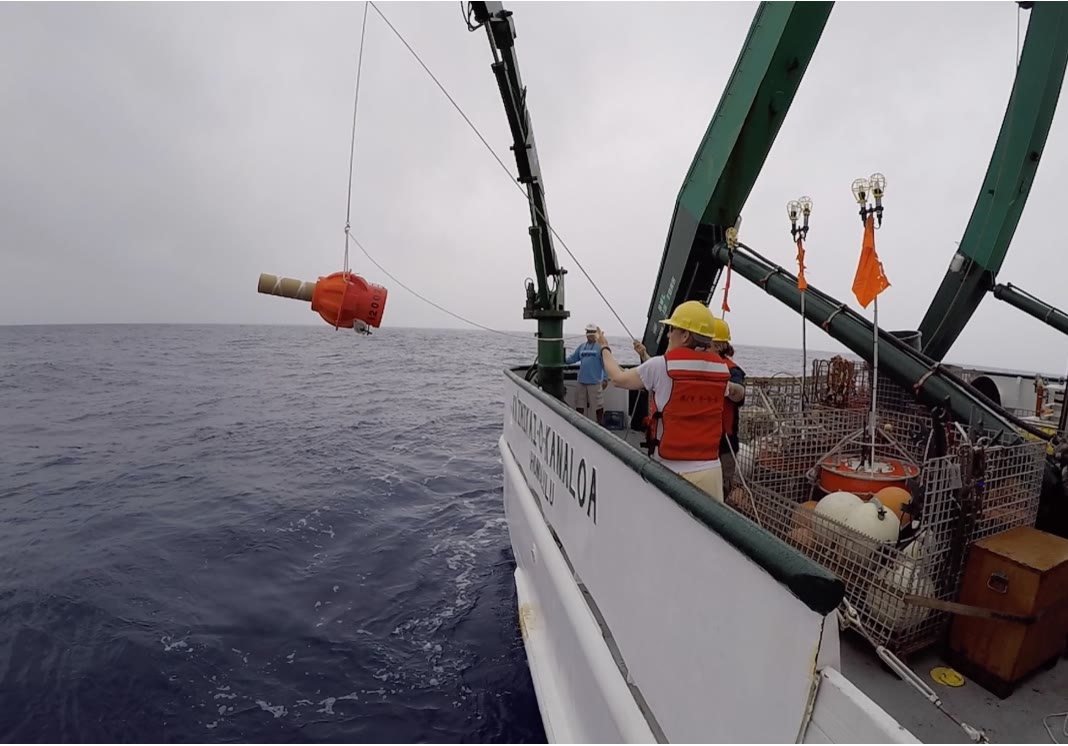
\includegraphics[width=0.6\linewidth]{images/book3/b1-deep-float.jpg}

{\small Um flutuador de perfilagem do oceano profundo (o instrumento laranja pendurado no guindaste)
sendo baixado de um navio de pesquisa em 2018; uma vez liberado, ele afunda até sua
profundidade de trabalho e volta à superfície em intervalos regulares para enviar seus dados. (Fotógrafo não
identificado da NOAA, domínio público, via Wikimedia Commons.)}
\label{fig:b1:ocean-circulation:float}
\end{omfigure}
% ledger: commons:deep-solo, noaa:argo-25

A circulação de revolvimento transporta calor. A água que vai para o norte quente e volta fria
cedeu calor à atmosfera do norte.

\begin{proposition}[Calor transportado por uma circulação de revolvimento]\label{prop:b1:ocean-circulation:heat}
Se um transporte volumétrico $Q$ cruza uma \omterm{def:b1:spherical-astronomy:geographic}{latitude} para o norte na \omterm{def:b1:fluid-envelopes-structure:potential-temperature}{temperatura potencial}
$\theta_1$ e retorna para o sul em $\theta_2$, sem transporte líquido de massa, a
circulação de revolvimento transporta para o norte o \omterm{def:b1:heat-budget:heat-flow}{fluxo de calor}
\[
  H = \rho c_p\,Q\,(\theta_1 - \theta_2),
\]
onde $c_p$ é o calor específico da água do mar.
\end{proposition}
% ledger: teos10:cp0

\begin{proof}
Cada segundo, a massa $\rho Q$ cruza para o norte levando o conteúdo de calor $\rho Q
c_p\theta_1$, contado a partir de um zero arbitrário de temperatura, e a mesma massa
cruza para o sul levando $\rho Q c_p\theta_2$. O fluxo líquido para o norte é a
diferença; como as duas massas são iguais, o zero arbitrário se cancela, e o
resultado é um transporte real de calor.
\end{proof}

Um balanço grosseiro do Atlântico Norte, feito por W.~Schmitz, dá à Corrente do Golfo
\qty{40}{\sverdrup} de água a \qty{18}{\celsius} para o norte, dos quais
\qty{14}{\sverdrup} retornam para o sul como água profunda a \qty{2}{\celsius}. Com $c_p =
\qty{3992}{J.kg^{-1}.K^{-1}}$ e $\rho = \qty{1027}{kg.m^{-3}}$, essa circulação de revolvimento
transporta $1027 \times 3992 \times \num{14e6} \times 16 = \qty{0.92e15}{W}$, cerca de
\qty{0.9}{PW}, para o norte de \ang{24} N; estimativas cuidadosas dão \qty{1.2}{PW}, um
quarto do transporte de calor para o polo feito pela atmosfera e pelo oceano
combinados. A maior parte desse calor é cedida ao ar sobre o Atlântico Norte setentrional,
o que é uma das razões pelas quais a Noruega, a \ang{60} N, é muito mais quente que o sul da
Groenlândia na mesma \omterm{def:b1:spherical-astronomy:geographic}{latitude}.
% ledger: stewart:heat-conveyor, rapid:home, teos10:cp0 (computed in calc/ch29.py)

A circulação profunda é lenta. Se leva cerca de mil anos para a água que afunda
no Atlântico Norte chegar ao Pacífico Norte pela Corrente Circumpolar Antártica,
sua velocidade média é de cerca de \qty{1}{mm/s}, cem vezes menor que as
correntes profundas variáveis que um correntômetro registra. Sua velocidade é, portanto, inferida
a partir de traçadores, e não medida: o trítio, liberado na atmosfera pelos testes
nucleares dos anos 1950 e decaindo com meia-vida de 12.3 anos, entrou no
Atlântico Norte profundo onde a água profunda se forma, e depois de 25 anos tinha se espalhado pouco
ao sul de \ang{30} N, uma velocidade média de menos de \qty{1}{mm/s}. O volume do oceano
dividido pela taxa em que a água profunda se forma dá a mesma ordem de tempo
(\cref{exo:b1:ocean-circulation:12}).
% ledger: stewart:deep-circulation, nos:conveyor

A Corrente Circumpolar Antártica une as bacias. Suas correntes atingem o fundo do mar
e são lentas, cerca de \qty{10}{cm/s}, até \qty{50}{cm/s} em suas frentes, mas é
profunda e larga: uma rede de correntômetros fundeados através da Passagem de Drake,
entre a América do Sul e a Antártida, deu \qty[uncertainty-mode=separate]{125 \pm
11}{\sverdrup} (publicado em 1985), e uma rede mais densa em 2007--2011,
que mediu também as correntes perto do fundo, deu \qty{173.3}{\sverdrup},
\qty{39}{\percent} a mais que aquele valor usado há muito tempo. Ela leva água profunda de cada
oceano aos outros e a mistura pelo caminho.
% ledger: stewart:acc, donohue:acc

\begin{dated}{2021}
% ledger: ipcc:amoc-observed, ipcc:amoc-projected
A avaliação de 2021 do Painel Intergovernamental sobre Mudanças Climáticas conclui, a partir de
reconstruções, que o revolvimento atlântico foi relativamente estável nos últimos
\num{8000} anos (\emph{confiança média}), com um enfraquecimento iniciado no fim do
século XIX (\emph{confiança média}), mas tem apenas \emph{baixa confiança} em um
declínio geral durante o século XX. O enfraquecimento observado diretamente de meados dos
anos 2000 a meados dos anos 2010 (\emph{alta confiança}) não pode ser distinguido da
variabilidade em escala de décadas (\emph{alta confiança}). É \emph{muito
provável} que o revolvimento se enfraqueça ao longo do século XXI em todos os cenários de emissões, com apenas
\emph{baixa confiança} quanto ao tamanho do declínio; há \emph{confiança média}
de que ele não entre em colapso abrupto antes de 2100.
\end{dated}

\section{Exercícios}

\begin{exercise}[$\star$]\label{exo:b1:ocean-circulation:1}
Use a fórmula de arrasto com $\rho_a = \qty{1.3}{kg.m^{-3}}$ e o coeficiente de arrasto
de Yelland e Taylor. (a)~Calcule $C_D$ e a \omterm{def:b1:ocean-circulation:wind-stress}{tensão do vento} para ventos de 4, 7 e
\qty{15}{m/s}. (b)~De que fator a tensão cresce de 7 a \qty{15}{m/s}?
Compare com a razão dos quadrados das velocidades e explique a diferença.
% ledger: stewart:wind-stress, stewart:drag-coefficient
\end{exercise}

\begin{exercise}[$\star$]\label{exo:b1:ocean-circulation:2}
Dê o sentido do \omterm{def:b1:ocean-circulation:ekman}{transporte de Ekman} em cada caso. (a)~Um vento soprando para leste a
\ang{45} N. (b)~Um alísio de nordeste a \ang{15} N.
(c)~Um vento soprando para leste a \ang{50} S. (d)~Um vento do sul ao longo da
costa oeste do sul da África, perto de \ang{23} S. Em qual dos quatro casos o
transporte aponta para o mar, e o que se segue disso?
\end{exercise}

\begin{exercise}[$\star$]\label{exo:b1:ocean-circulation:3}
A \ang{26.5} N no Atlântico, os transportes médios de 2004--2024 são: Estreito da
Flórida \qty{31.7}{\sverdrup}, Ekman \qty{3.5}{\sverdrup}, oceano médio superior
\qty{-17.9}{\sverdrup}; por camadas, 0--\qty{800}{m} \qty{16.6}{\sverdrup},
800--\qty{1100}{m} \qty{0.4}{\sverdrup}, 1100--\qty{3000}{m} \qty{-12.0}{\sverdrup},
3000--\qty{5000}{m} \qty{-5.9}{\sverdrup} (positivo para o norte). (a)~Some as três
primeiras e compare com o revolvimento publicado, \qty{17.1}{\sverdrup}. (b)~Compare
o fluxo para o norte acima de \qty{1100}{m} com o fluxo para o sul abaixo. (c)~Converta
\qty{17.1}{\sverdrup} em quilômetros cúbicos por ano, e calcule o tempo que este fluxo
levaria para encher o volume de todo o oceano, \qty{1.3324e9}{km^3}.
% ledger: rapid:transports, charette:ocean-volume
\end{exercise}

\begin{exercise}[$\star$]\label{exo:b1:ocean-circulation:4}
Com as fórmulas de Ekman, calcule a profundidade de Ekman e a corrente de superfície sob um
vento de \qty{10}{m/s} a \ang{15}, \ang{45} e \ang{60} de \omterm{def:b1:spherical-astronomy:geographic}{latitude}, e a
corrente de superfície como porcentagem do vento. Por que as fórmulas falham perto do equador?
% ledger: stewart:ekman-constants
\end{exercise}

\begin{exercise}[$\star\star$]\label{exo:b1:ocean-circulation:5}
Ao longo de \ang{11} N no Atlântico, tome uma tensão média do vento de \qty{0.07}{Pa} para
oeste em uma largura de \qty{5000}{km}, e $\rho = \qty{1027}{kg.m^{-3}}$.
(a)~Calcule o \omterm{def:b1:ocean-circulation:ekman}{transporte de Ekman} por metro e seu sentido. (b)~Calcule o
transporte volumétrico total através da seção, em \omterm{def:b1:ocean-circulation:ekman}{sverdrups}. (c)~Compare com os transportes
medidos diretamente ($12.0 \pm \qty{5.5}{\sverdrup}$) e calculados a partir de
ventos de longo prazo ($13.5 \pm \qty{0.3}{\sverdrup}$).
% ledger: stewart:ekman-transport
\end{exercise}

\begin{exercise}[$\star\star$]\label{exo:b1:ocean-circulation:6}
Ao longo do Pacífico equatorial, os \omterm{def:b1:atmospheric-circulation:winds}{alísios} exercem uma tensão de \qty{0.05}{Pa}
para oeste. (a)~Calcule o \omterm{def:b1:ocean-circulation:ekman}{transporte de Ekman} por metro, e seu sentido, a
\ang{2} N e a \ang{2}~S. (b)~Supondo que a água levada para longe nestas duas
\omterm{def:b1:spherical-astronomy:geographic}{latitudes} seja reposta por baixo entre elas, calcule a velocidade média de \omterm{def:b1:ocean-circulation:upwelling}{ressurgência}
em metros por dia. (c)~O que acontece com a fórmula do teorema no próprio equador?
Qual conclusão sobrevive?
\end{exercise}

\begin{exercise}[$\star\star$]\label{exo:b1:ocean-circulation:7}
Sobre um \omterm{def:b1:ocean-circulation:gyre}{giro subtropical}, tome uma \omterm{def:b1:ocean-circulation:wind-stress}{tensão do vento} de \qty{0.06}{Pa} para oeste a
\ang{15} N e \qty{0.12}{Pa} para leste a \ang{40} N. (a)~Calcule ambos os \omterm{def:b1:ocean-circulation:ekman}{transportes de
Ekman} e seus sentidos. (b)~Supondo que o transporte varia uniformemente entre as
duas \omterm{def:b1:spherical-astronomy:geographic}{latitudes}, calcule a velocidade vertical na base da \omterm{def:b1:ocean-circulation:ekman}{camada de Ekman}, em
metros por ano, e diga se ela é para cima ou para baixo. (c)~Sobre uma bacia de
\qty{5000}{km} de largura, quantos \omterm{def:b1:ocean-circulation:ekman}{sverdrups} são bombeados através da base da camada?
\end{exercise}

\begin{exercise}[$\star\star$]\label{exo:b1:ocean-circulation:8}
Tome $\rho = \qty{1027}{kg.m^{-3}}$ e $c_p = \qty{3992}{J.kg^{-1}.K^{-1}}$.
(a)~Calcule o calor transportado para o norte por \qty{17}{\sverdrup} fluindo para o norte a
\qty{15}{\celsius} e retornando a \qty{3}{\celsius}. (b)~Compare com o
\qty{1.2}{PW} transportado pelo revolvimento atlântico. (c)~Se a mesma água retornasse
para o sul na superfície, ao longo do lado leste da bacia, a \qty{12}{\celsius},
que calor ela transportaria? O que isso diz sobre a importância da
\omterm{def:b1:ocean-circulation:moc}{formação de água profunda}?
% ledger: rapid:home, teos10:cp0
\end{exercise}

\begin{exercise}[$\star\star$]\label{exo:b1:ocean-circulation:9}
Três \omterm{def:b1:fluid-envelopes-structure:ts-diagram}{massas de água} do Atlântico Sul têm as temperaturas potenciais e
salinidades: Água Intermediária Antártica \qty{3.3}{\celsius}, 34.15; Água Profunda do
Atlântico Norte \qty{4.0}{\celsius}, 35.00; Água de Fundo Antártica \qty{0.4}{\celsius},
34.67. Uma amostra em profundidade tem $\theta = \qty{2.78}{\celsius}$ e $S = 34.731$.
Usando \cref{prop:b1:fluid-envelopes-structure:mixing}, encontre a fração de cada
\omterm{def:b1:fluid-envelopes-structure:ts-diagram}{massa de água} na amostra.
% ledger: stewart:deep-circulation
\end{exercise}

\begin{exercise}[$\star\star\star$]\label{exo:b1:ocean-circulation:10}
Tome a espiral de \cref{prop:b1:ocean-circulation:spiral}. (a)~Mostre que $u$ e $v$
satisfazem $f v + A_z u'' = 0$ e $-f u + A_z v'' = 0$. (Dica: escreva $u + iv =
V_0\,e^{i\pi/4}\,e^{(1+i)az}$.) (b)~Mostre que a tensão $\rho A_z\,\partial\vec
v/\partial z$ na superfície é igual à \omterm{def:b1:ocean-circulation:wind-stress}{tensão do vento} $(0, T)$. (c)~Calcule os
transportes $\int_{-\infty}^0 \rho u\,\mathrm dz$ e $\int_{-\infty}^0 \rho
v\,\mathrm dz$, e verifique que eles concordam com
\cref{thm:b1:ocean-circulation:ekman}.
\end{exercise}

\begin{exercise}[$\star\star\star$]\label{exo:b1:ocean-circulation:11}
No modelo de Stommel, a \omterm{def:b1:ocean-circulation:wbc}{corrente de contorno oeste} tem uma largura de cerca de $R/\beta$,
em que $R$ é a taxa de atrito no fundo e $\beta = \mathrm df/\mathrm dy$ a
taxa de crescimento para o norte do \omterm{def:b1:atmospheric-circulation:coriolis-parameter}{parâmetro de Coriolis}. (a)~Mostre que $\beta = 2\Omega
\cos\varphi/a_\oplus$ e calcule-o a \ang{30} N ($a_\oplus = \qty{6371}{km}$).
(b)~Com $R = \qty{e-6}{s^{-1}}$, calcule a largura. (c)~Um transporte de
\qty{30}{\sverdrup} deriva para o sul através do interior de uma bacia de \qty{5000}{km} de largura
na parte superior de \qty{1000}{m}, e retorna para o norte na corrente de contorno na mesma
profundidade. Calcule ambas as velocidades médias e compare com a velocidade da Corrente do Golfo,
\qty{1.8}{m/s}.
% ledger: stewart:north-atlantic, nos:gulf-stream, earth:Rmean
\end{exercise}

\begin{exercise}[$\star\star\star$]\label{exo:b1:ocean-circulation:12}
O oceano contém \qty{1.3324e9}{km^3} sobre \qty{361.84e6}{km^2}. (a)~Mostre que o
volume abaixo de \qty{1000}{m} é de pelo menos \qty{9.71e8}{km^3}. (b)~A Água Profunda do
Atlântico Norte se forma a cerca de \qty{17}{\sverdrup} e a Água de Fundo Antártica a cerca de
\qty{9}{\sverdrup}. Estime o tempo necessário para renovar a água abaixo de
\qty{1000}{m}, e compare com os mil anos da correia transportadora. (c)~O trítio tem uma
meia-vida de 12.3 anos. Que fração de uma entrada de trítio resta após 25 anos? A que
distância viaja a água que se move a \qty{1}{mm/s} em 25 anos?
% ledger: charette:ocean-volume, stewart:deep-circulation, stewart:acc, rapid:transports
\end{exercise}

\section{Problema: uma costa de ressurgência}

\begin{problem}[{Problema de fim de semana --- um vento de verão ao longo de uma costa a \ang{38} N}]
\label{pb:b1:ocean-circulation:1}
% values: calc/ch29.py (invented coast; constants from the ledger)
Uma costa retilínea corre norte--sul a \ang{38} N, com o oceano a oeste. No
verão, um vento permanente de \qty{8}{m/s} sopra do norte ao longo dela por semanas. A
costa é inventada, mas seus números são típicos dos lados leste dos oceanos.
Use $\Omega = 2\pi/(\qty{23.9345}{h})$, $\rho_a = \qty{1.3}{kg.m^{-3}}$, o coeficiente de arrasto
de Yelland e Taylor, $\rho = \qty{1027}{kg.m^{-3}}$ para a água do mar e
$c_p = \qty{3992}{J.kg^{-1}.K^{-1}}$.

\medskip
\noindent\textbf{Parte I --- O vento e sua tensão.}
\begin{enumerate}
  \item Em qual direção sopra o vento? Ele é ao longo da costa ou através
        dela?
  \item Calcule o coeficiente de arrasto.
  \item Calcule a \omterm{def:b1:ocean-circulation:wind-stress}{tensão do vento}.
  \item Mesmas duas perguntas para um vento de \qty{12}{m/s}. De que fator a
        tensão cresce, e por que ele é maior que a razão dos quadrados das velocidades?
  \item Calcule o \omterm{def:b1:atmospheric-circulation:coriolis-parameter}{parâmetro de Coriolis} a \ang{38} N.
  \item Calcule $2\pi/f$ em horas. Por que o vento deve soprar por um dia ou mais antes
        que o equilíbrio de Ekman se aplique?
\end{enumerate}

\medskip
\noindent\textbf{Parte II --- A camada de Ekman.}
\begin{enumerate}[resume]
  \item Em qual direção está o \omterm{def:b1:ocean-circulation:ekman}{transporte de Ekman}? Em direção à terra ou ao mar aberto?
  \item Calcule o transporte de massa de Ekman por metro de costa.
  \item Converta-o em transporte volumétrico por metro.
  \item Calcule a profundidade de Ekman com a fórmula de Ekman.
  \item Calcule a velocidade média para o mar na camada, em \unit{cm/s}.
  \item Calcule a corrente de superfície com a fórmula de Ekman, e seu sentido. O que
        as medidas de derivadores sugerem para a sua velocidade?
\end{enumerate}

\medskip
\noindent\textbf{Parte III --- Ressurgência na costa.}
\begin{enumerate}[resume]
  \item Explique, com um esboço de uma seção vertical, de onde vem a água levada
        para o mar.
  \item Calcule o volume ressurgido por dia ao longo de cada quilômetro de costa.
  \item Suponha que a água suba por uma faixa de \qty{20}{km} de largura ao longo da
        costa. Calcule a velocidade média para cima, em \unit{m/s} e em metros por dia.
  \item Quanto tempo leva para a água subir da base da \omterm{def:b1:ocean-circulation:ekman}{camada de Ekman} até a
        superfície nesta velocidade?
  \item A água ressurgida chega à superfície a \qty{12}{\celsius}, enquanto o mar aberto
        ao largo está a \qty{18}{\celsius}. A brisa marítima leva ar quente e úmido do
        mar aberto sobre essa água. O que acontece com o ar perto da superfície, e que
        tempo se segue na costa?
  \item Por que essas costas são ricas em peixes?
  \item No outono o vento gira e sopra do sul por uma semana. O que acontece
        com o transporte e com a água na costa?
\end{enumerate}

\medskip
\noindent\textbf{Parte IV --- Outras costas e o transporte total.}
\begin{enumerate}[resume]
  \item Com a mesma tensão, calcule o \omterm{def:b1:ocean-circulation:ekman}{transporte de Ekman} por metro a \ang{20} N
        e compare com \ang{38} N.
  \item Na costa oeste do sul da África, perto de \ang{23} S, qual direção do vento
        impulsiona a \omterm{def:b1:ocean-circulation:upwelling}{ressurgência}? Compare com a costa do problema.
  \item Sob um vento de \qty{5}{m/s} em vez de \qty{8}{m/s} a \ang{38} N, calcule
        a tensão e o \omterm{def:b1:ocean-circulation:ekman}{transporte de Ekman} por metro, e a razão deles com os de
        a pergunta~8.
  \item A água ressurgida aquece \qty{6}{\celsius} ao derivar para o mar aberto. Calcule
        o calor que ela absorve por segundo por metro de costa, e depois ao longo de
        \qty{1000}{km}.
  \item Que comprimento de tal costa ressurgiria tanta água quanto a Corrente do Golfo
        transporta pelo Estreito da Flórida, \qty{31.7}{\sverdrup}?
  \item Que volume de água, em \omterm{def:b1:ocean-circulation:ekman}{sverdrups}, é ressurgido ao longo de \qty{1000}{km} desta
        costa?
\end{enumerate}
\end{problem}
